
\par $S_{cheio} = [2,4]$

\vskip 0.1in
\par $S_{alternativa^+} = [2,3]$   \qquad $S_{alternativa^-} = [0,1]$
\par $Ganho(S_{cheio}, S_{alternativa}) = 0.109$

\vskip 0.1in
\par $S_{bar^+} = [1,2]$  \qquad $S_{bar^-} = [1,2]$
\par $Ganho(S_{cheio}, S_{bar}) = 0$

\vskip 0.1in
\par $S_{fimSemana^+} = [2,3]$  \qquad $S_{fimSemana^-} = [0,1]$
\par $Ganho(S_{cheio}, S_{fimSemana}) = 0.109$

\vskip 0.1in
\par $S_{fome^+} = [2,2]$ \qquad   $S_{fome^-} = [0,2]$
\par $Ganho(S_{cheio}, S_{fome}) = 0.251$

\vskip 0.1in
\par $S_{preco^{S}} = [2,2]$ \qquad $S_{preco^{SSS}} = [0,2]$
\par $Ganho(S_{cheio}, S_{preco}) = 0.251$

\vskip 0.1in
\par $S_{chuva^{+}} = [1,1]$  \qquad $S_{chuva^{-}} = [1,3]$
\par $Ganho(S_{cheio}, S_{chuva}) = 0.044$

\vskip 0.1in
\par $S_{reserva^{+}} = [0,2]$  \qquad $S_{reserva^{-}} = [2,2]$
\par $Ganho(S_{cheio}, S_{reserva}) = 0.25$

\vskip 0.5in
\par $S_{tipo^{Fra}} = [0,1]$  \qquad $S_{tipo^{Tai}} = [1,1]$ 
    \qquad $S_{tipo^{Ita}} = [0,1]$ \qquad $S_{tipo^{Ham}} = [1,1]$ 
\par $Ganho(S_{cheio}, S_{tipo}) = 0.251$

\vskip 0.1in
\par $S_{tespera^{10-30}} = [1,1]$ \qquad $S_{tespera^{30-60}} = [1,1]$ \qquad $S_{tespera^{>60}} = [0,2]$ 
\par $Ganho(S_{cheio_{fome}}, S_{tespera}) = 0.251$

\vskip 0.25in
\hfil
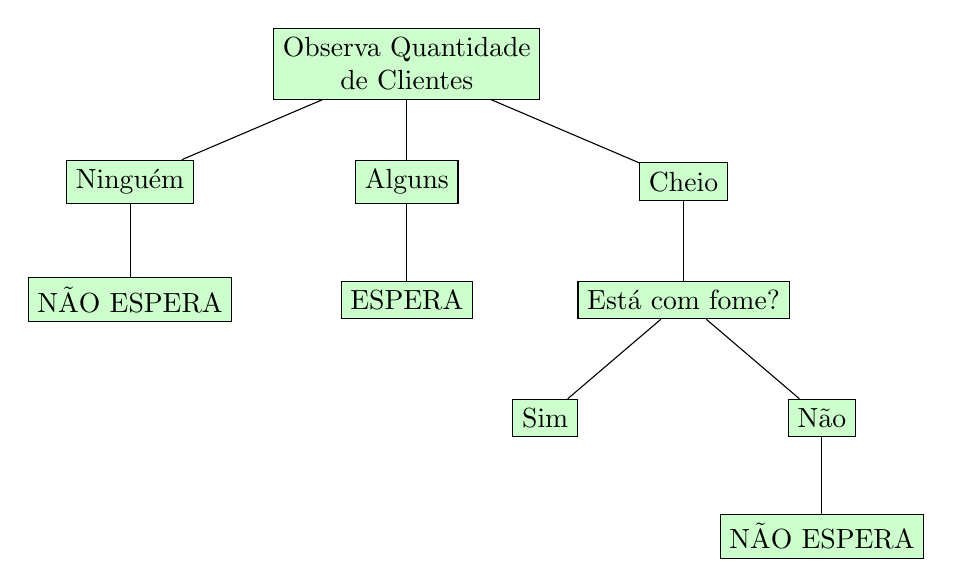
\begin{tikzpicture}[sibling distance=10em,
    every node/.style = {shape=rectangle, 
      draw, align=center,
      top color=green!20, bottom color=green!20}]]
    \node {Observa Quantidade \\ de Clientes}
        child { node {Ninguém} child { node {NÃO ESPERA}  } }
        child { node {Alguns} child { node {ESPERA}  } }
        child { node {Cheio} child { 
            node {Está com fome?} child { node {Sim}  } child { node {Não} child { node {NÃO ESPERA}  }  }
            }
        };
  \end{tikzpicture}